% Generated by julia/scripts/analyze_algorithmic_compression_v2.jl
\begin{figure}[tbp]
  \centering
  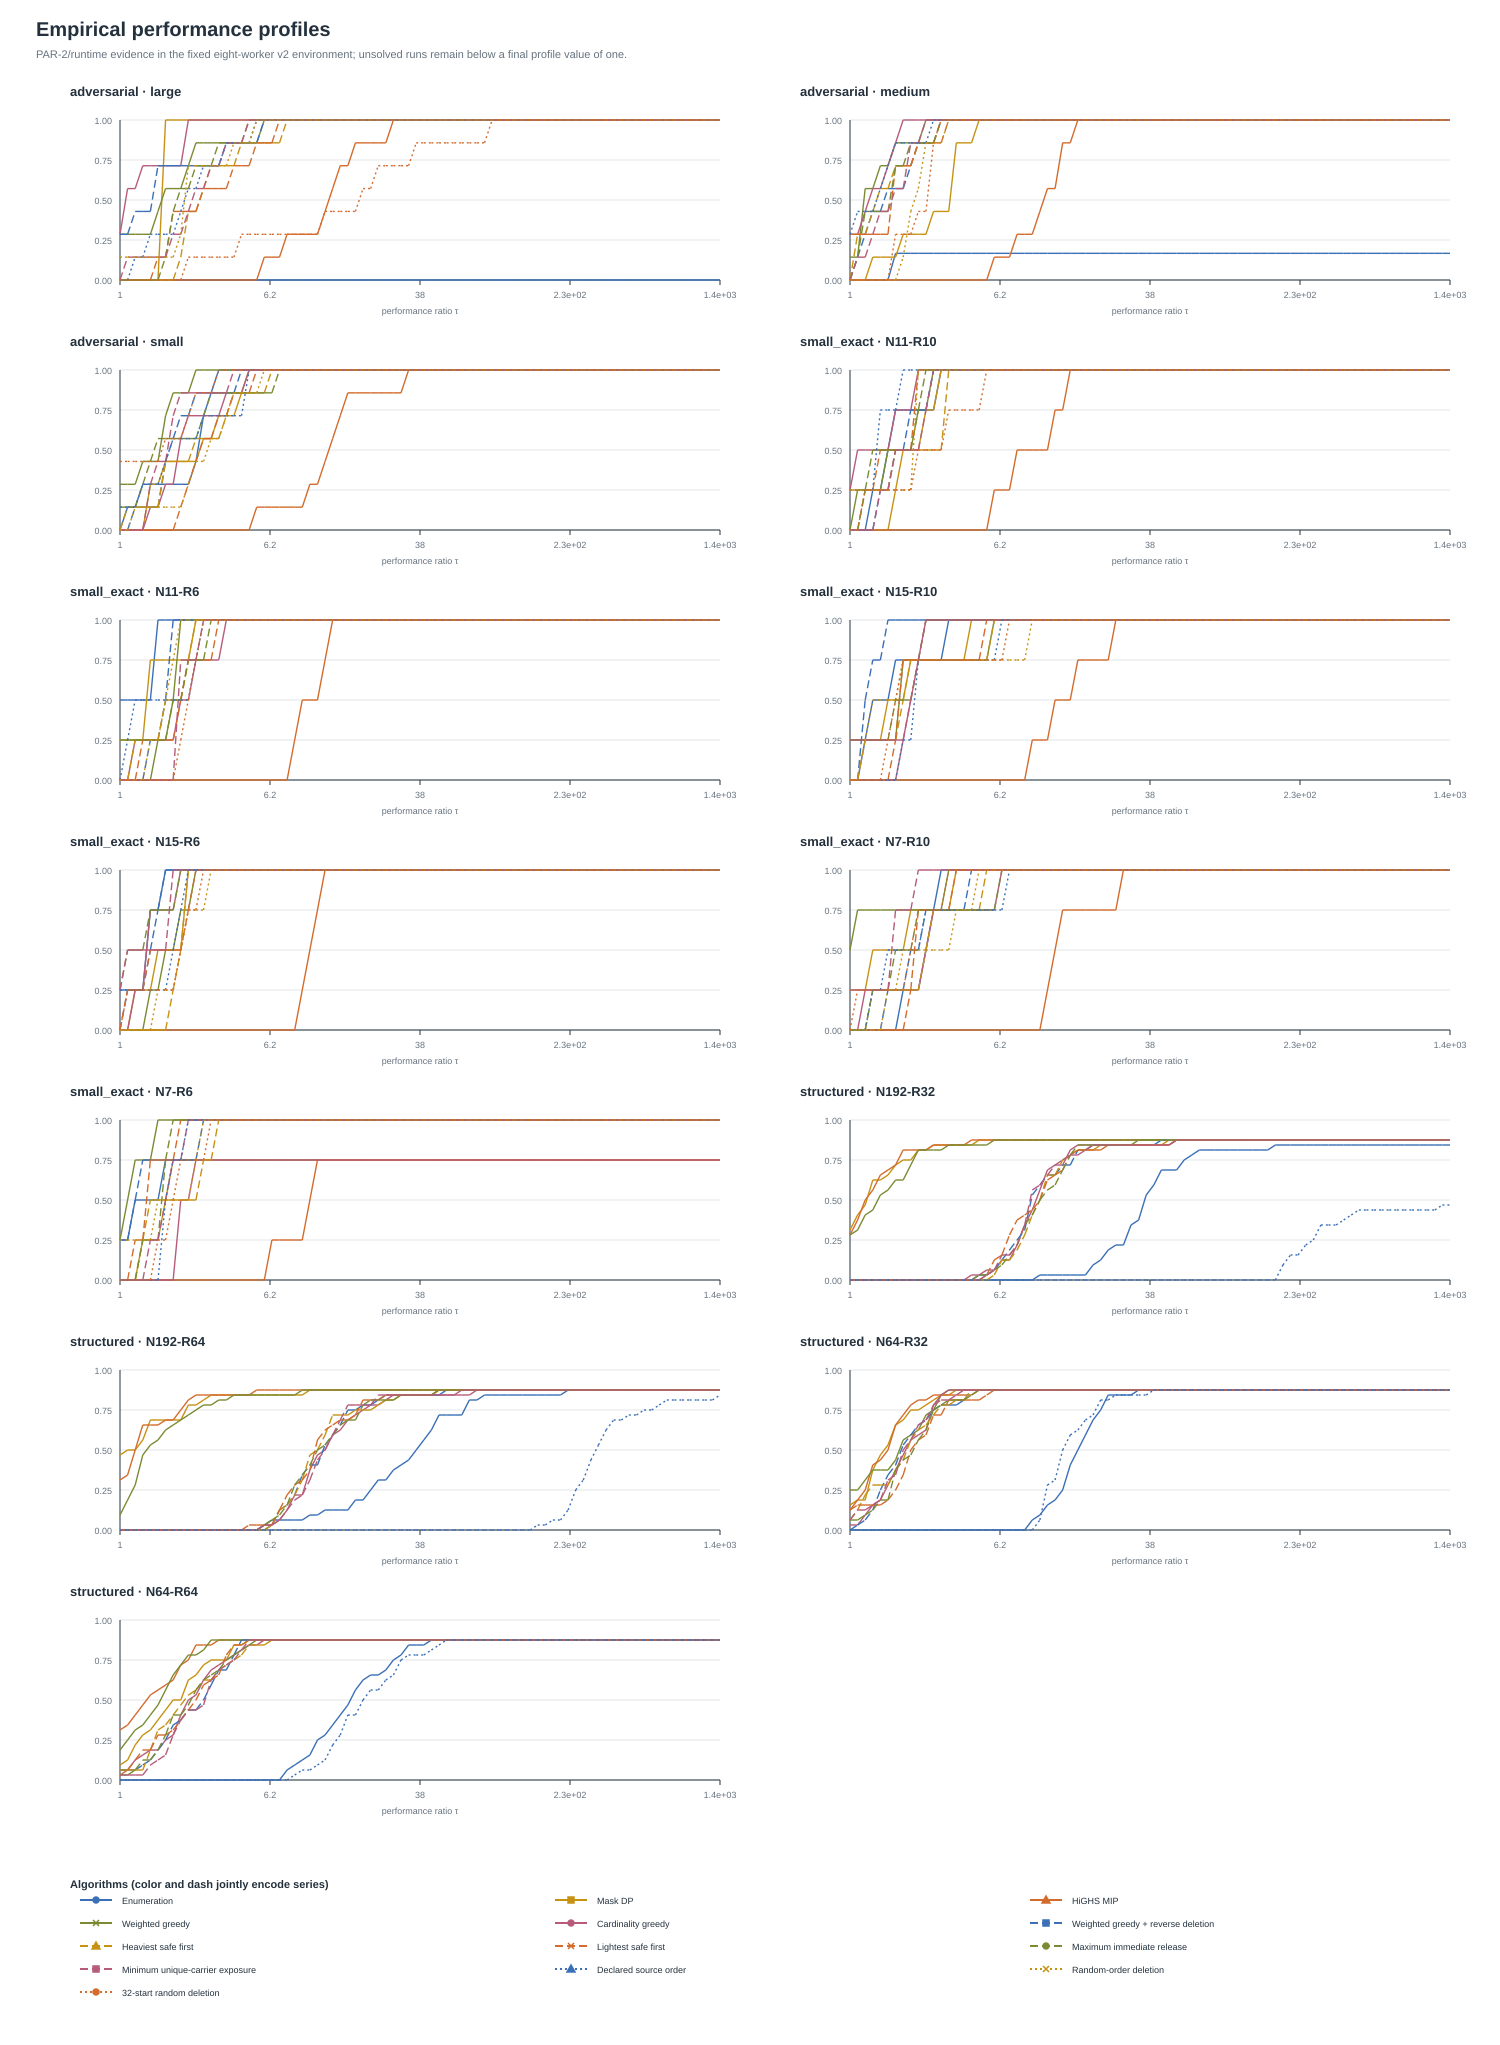
\includegraphics[width=\linewidth]{journal/aor/figures/performance_profile.svg}
  \caption{Synthetic performance profiles under the fixed eight-worker v2 environment. Unsuccessful runs remain in method denominators; the figure is computational evidence, not an algorithmic guarantee.}
  \label{fig:aor-performance-profile}
\end{figure}

\begin{figure}[tbp]
  \centering
  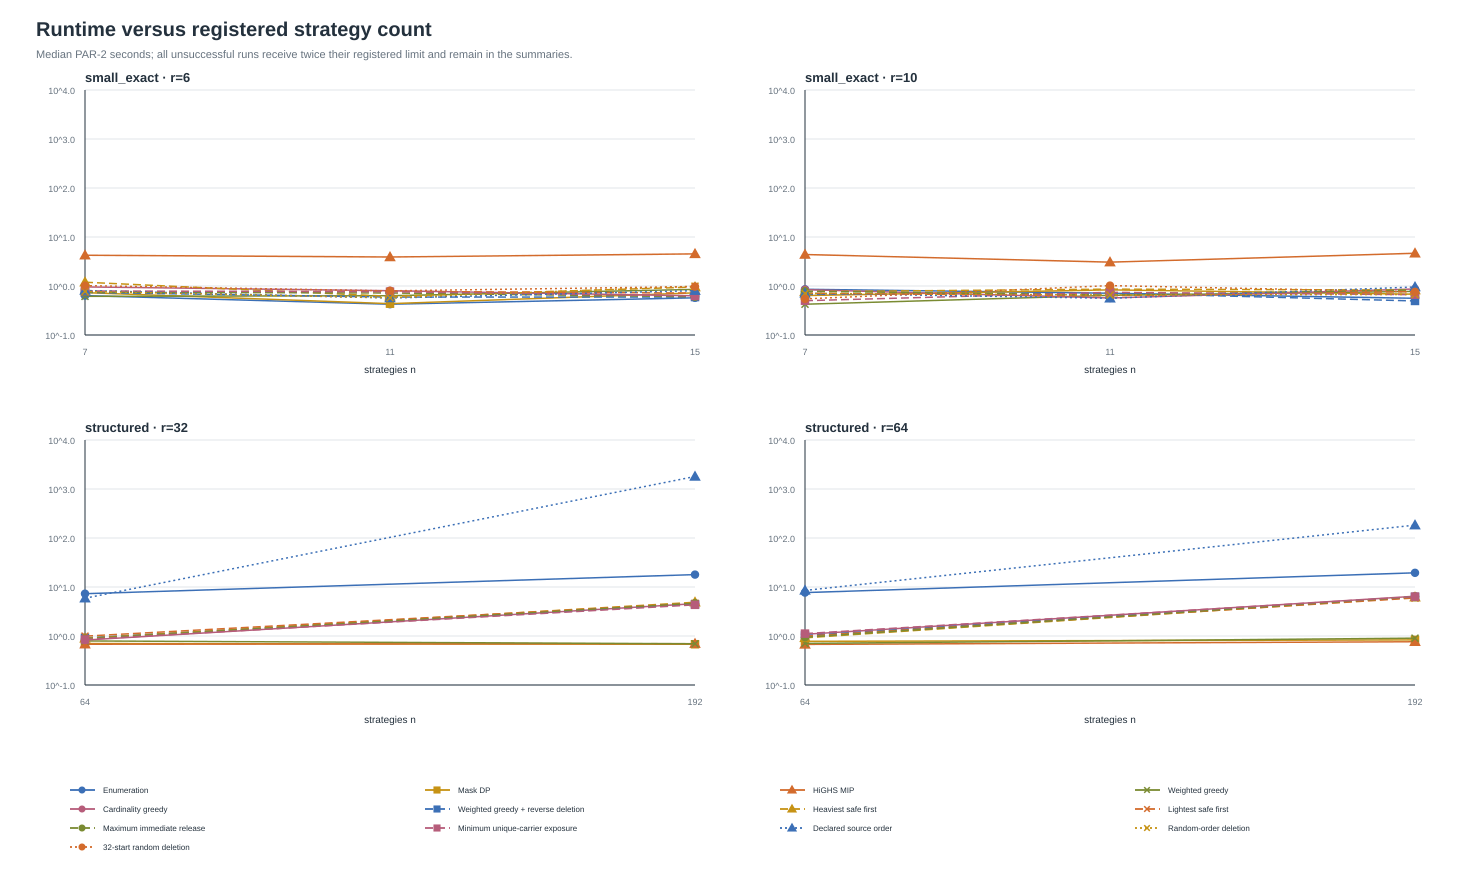
\includegraphics[width=\linewidth]{journal/aor/figures/runtime_vs_size.svg}
  \caption{Median PAR-2 runtime across registered size cells. Values are synthetic experimental measurements conditional on the declared hardware and concurrency.}
  \label{fig:aor-runtime-vs-size}
\end{figure}

\begin{figure}[tbp]
  \centering
  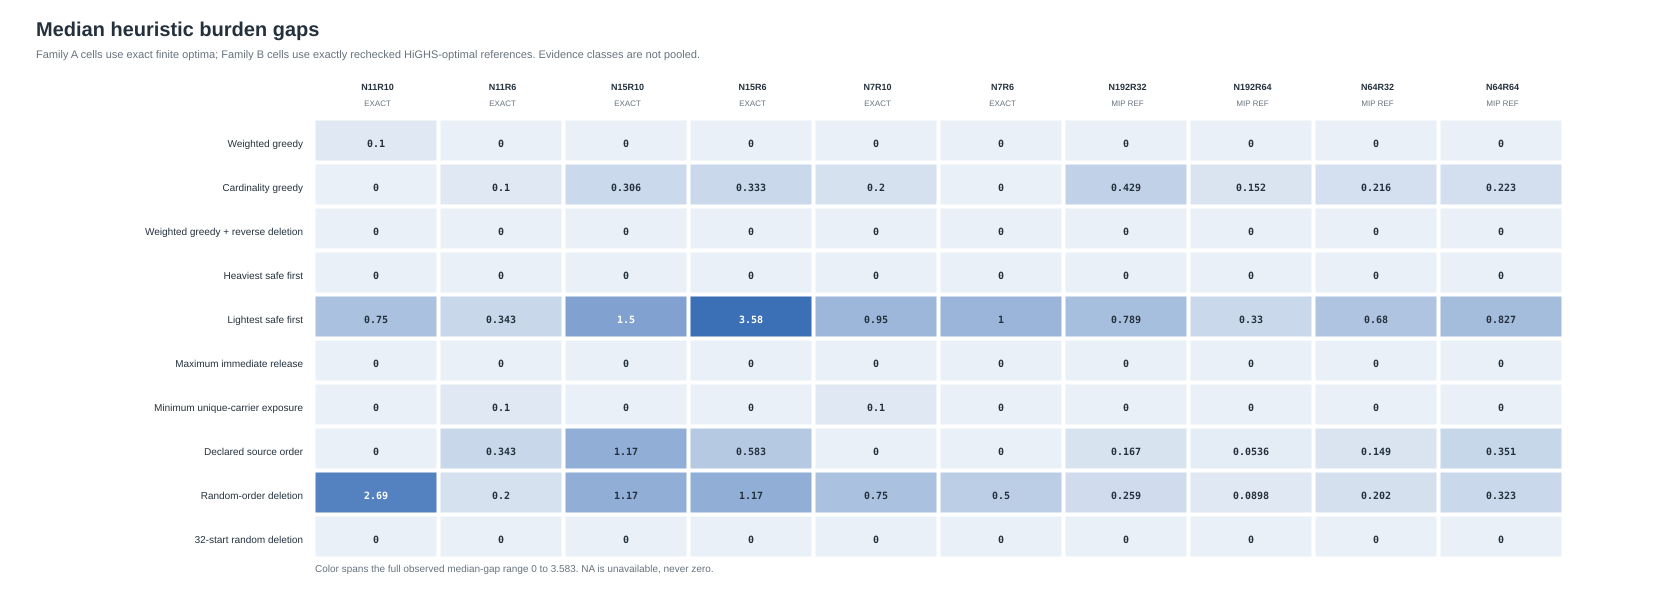
\includegraphics[width=\linewidth]{journal/aor/figures/heuristic_gap_heatmap.svg}
  \caption{Median heuristic burden gaps. Family A uses exact finite optima; Family B uses exactly rechecked HiGHS-optimal references, which are solver evidence rather than formal proof.}
  \label{fig:aor-heuristic-gap-heatmap}
\end{figure}

\begin{figure}[tbp]
  \centering
  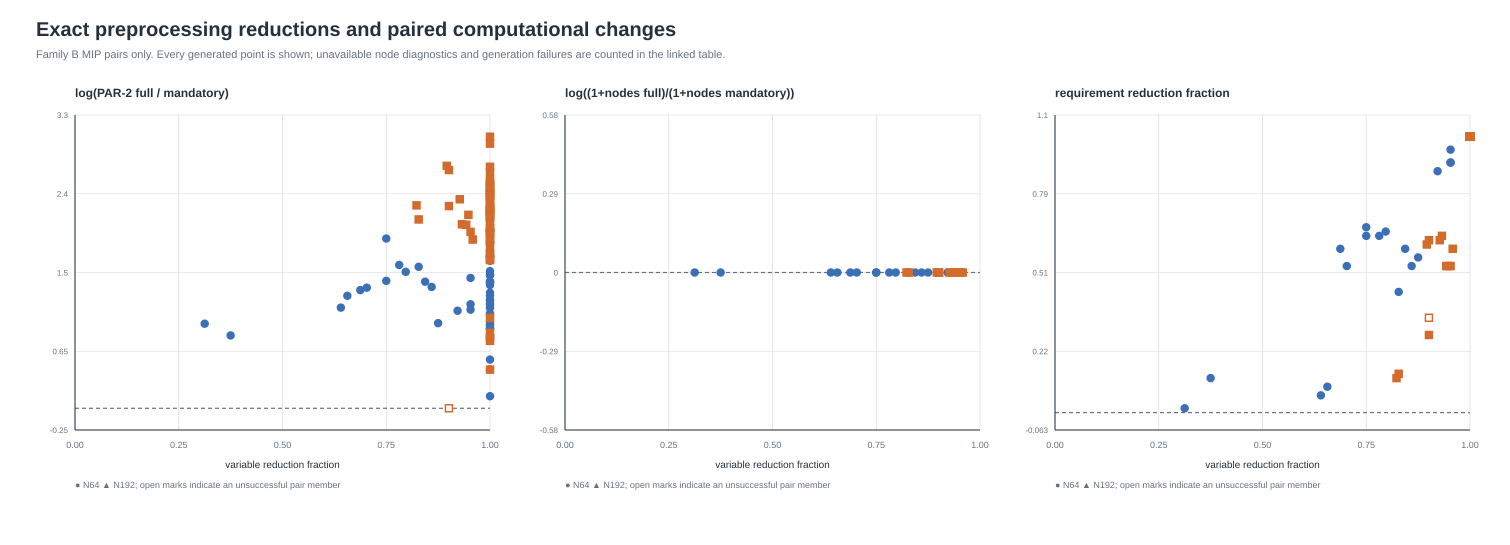
\includegraphics[width=\linewidth]{journal/aor/figures/preprocessing_reduction.svg}
  \caption{Exact preprocessing reductions and paired computational changes. Reconstruction and feasibility are exact finite checks; runtime and node changes are synthetic experimental evidence.}
  \label{fig:aor-preprocessing-reduction}
\end{figure}

\begin{figure}[tbp]
  \centering
  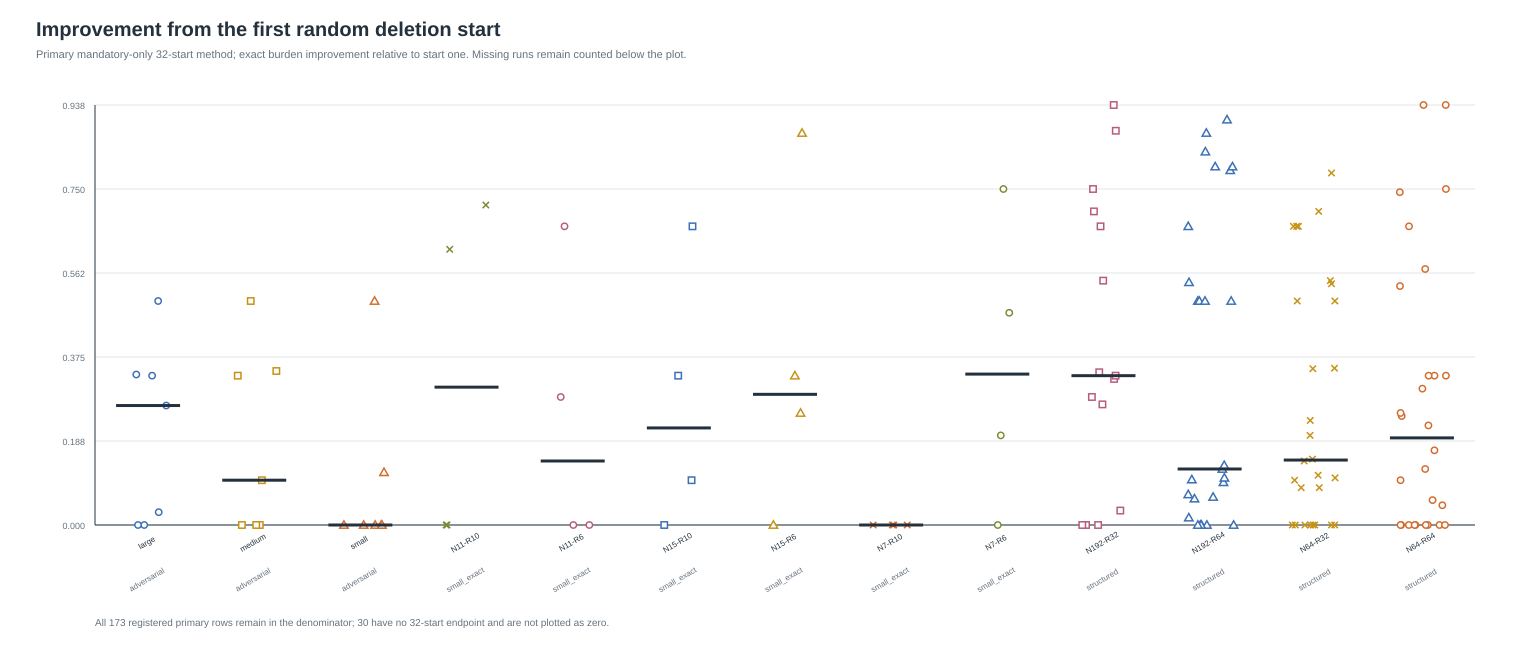
\includegraphics[width=\linewidth]{journal/aor/figures/multistart_improvement.svg}
  \caption{Exact burden improvement of registered 32-start deletion over start one. The endpoints are exactly feasible finite computations; their distribution is synthetic evidence.}
  \label{fig:aor-multistart-improvement}
\end{figure}

\begin{figure}[tbp]
  \centering
  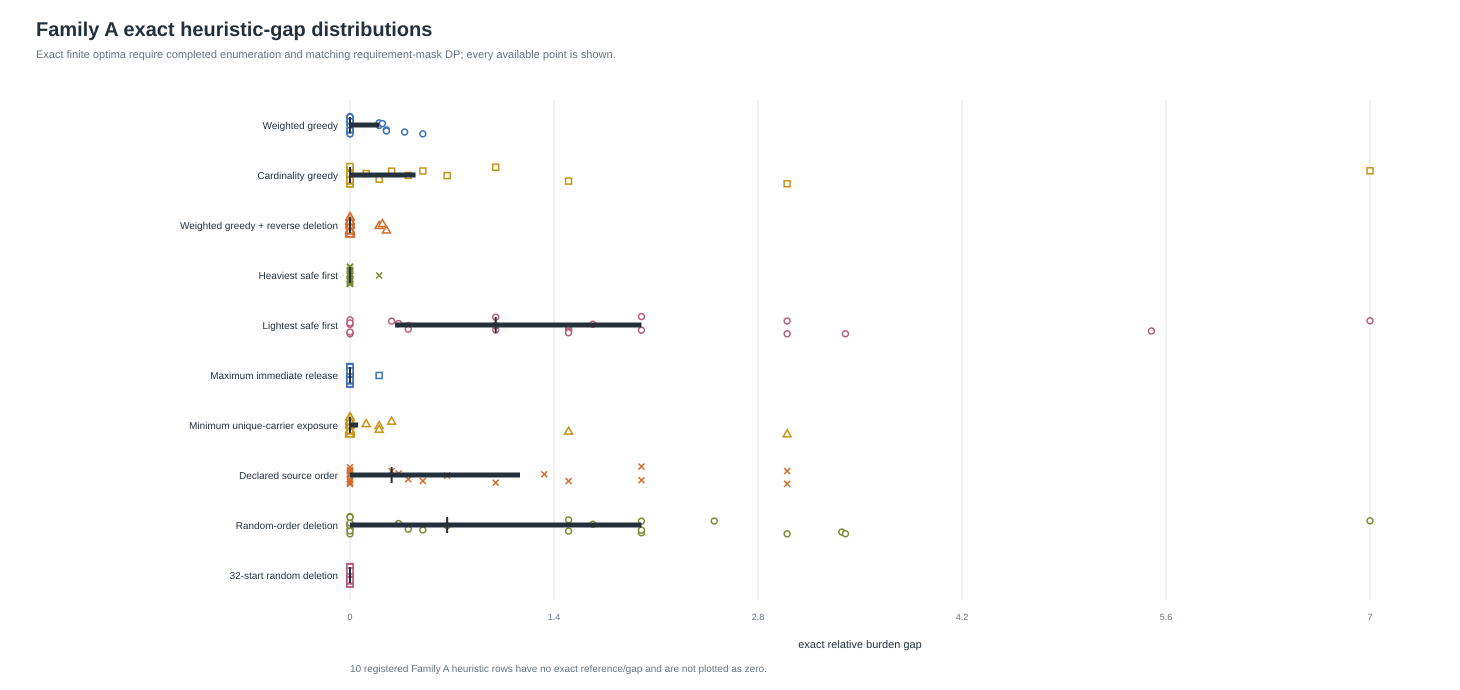
\includegraphics[width=\linewidth]{journal/aor/figures/family_a_exact_gap_distributions.svg}
  \caption{Family A heuristic gaps relative to optima established by agreeing complete finite methods. This is exact finite computation, not Lean verification.}
  \label{fig:aor-family-a-exact-gap-distributions}
\end{figure}

\begin{figure}[tbp]
  \centering
  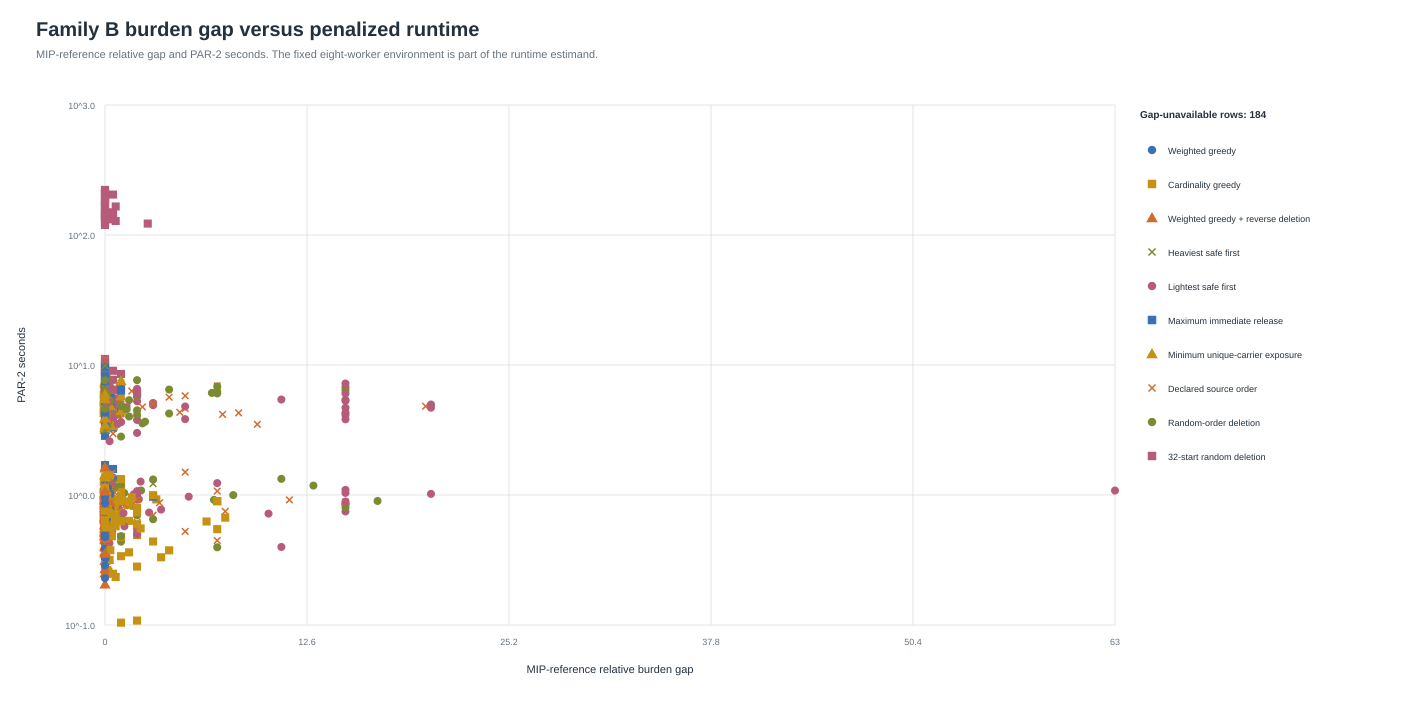
\includegraphics[width=\linewidth]{journal/aor/figures/family_b_burden_runtime_frontier.svg}
  \caption{Family B burden quality against PAR-2. Burden references are exactly rechecked HiGHS-optimal incumbents; runtime is eight-worker synthetic evidence.}
  \label{fig:aor-family-b-burden-runtime-frontier}
\end{figure}

\begin{figure}[tbp]
  \centering
  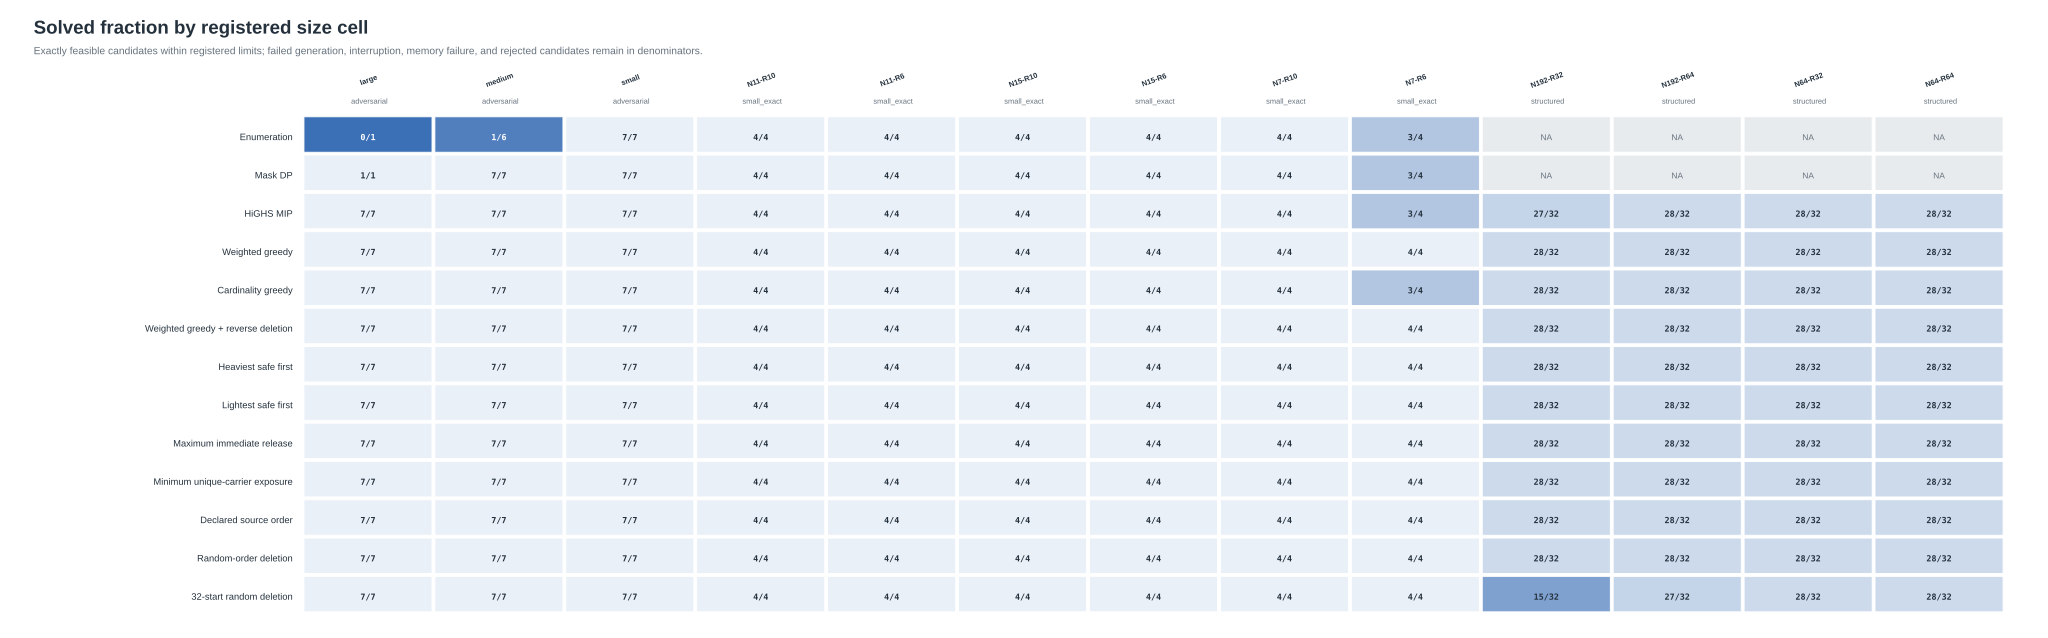
\includegraphics[width=\linewidth]{journal/aor/figures/solved_fraction_grid.svg}
  \caption{Solved fractions with all registered failures retained. This is synthetic experimental evidence under registered limits.}
  \label{fig:aor-solved-fraction-grid}
\end{figure}

\begin{figure}[tbp]
  \centering
  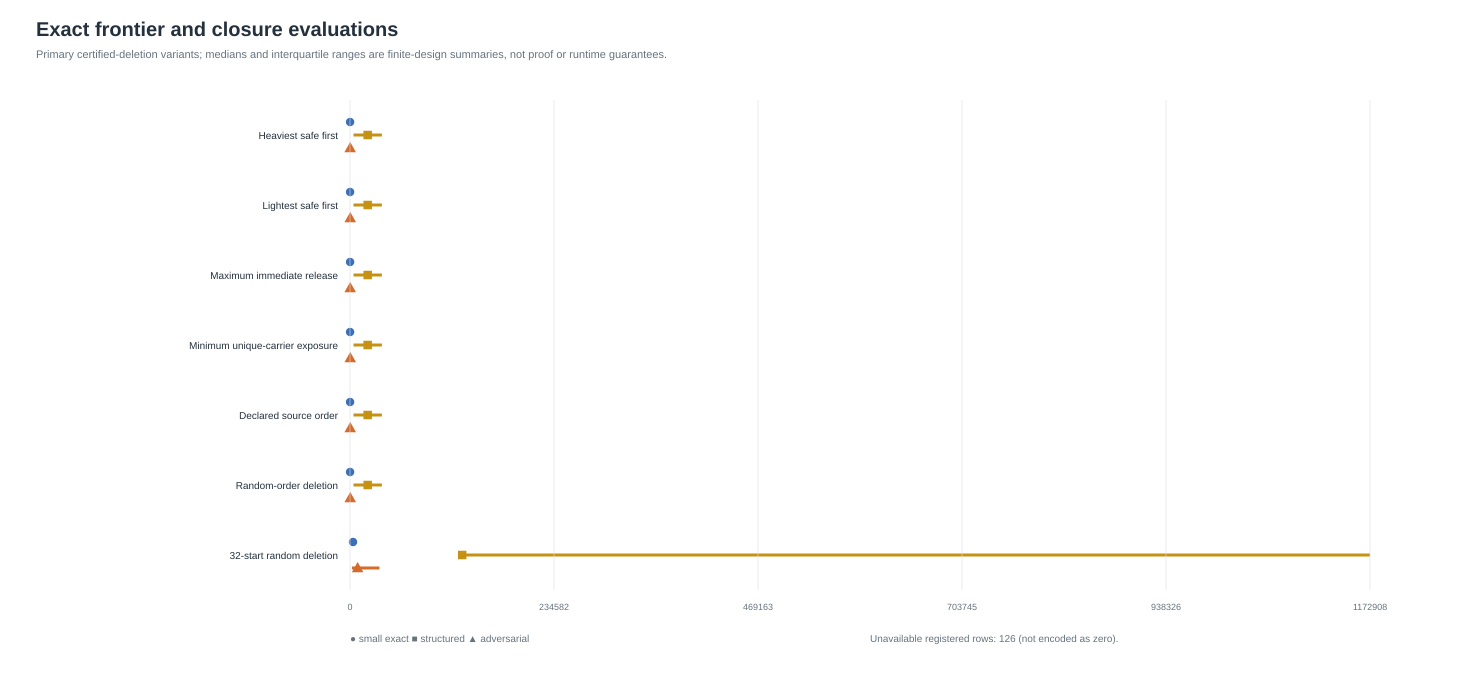
\includegraphics[width=\linewidth]{journal/aor/figures/semantic_evaluation_counts.svg}
  \caption{Exact frontier and closure evaluation counts for certified deletion. Counts are computational measurements and do not prove an approximation factor.}
  \label{fig:aor-semantic-evaluation-counts}
\end{figure}

\begin{figure}[tbp]
  \centering
  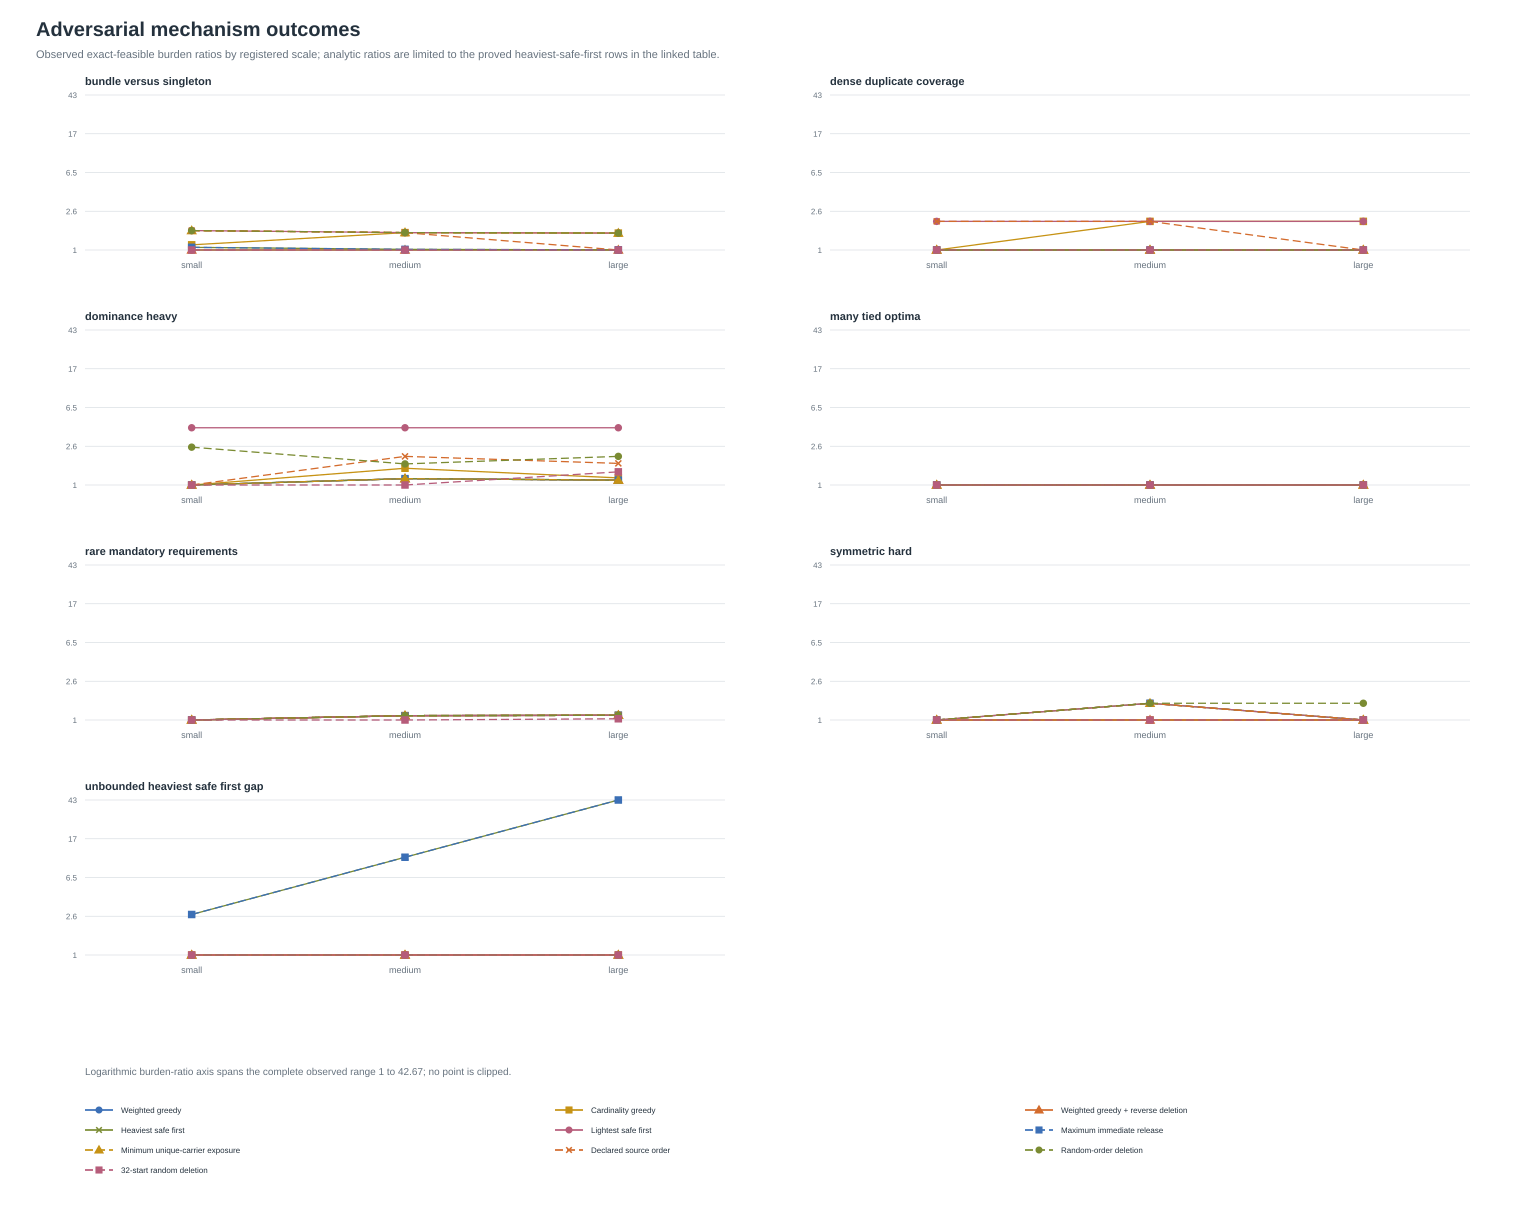
\includegraphics[width=\linewidth]{journal/aor/figures/adversarial_mechanisms.svg}
  \caption{Adversarial synthetic burden ratios. Only the registered heaviest-safe-first family has a separate human proof for its analytic ratio; other curves are finite computation.}
  \label{fig:aor-adversarial-mechanisms}
\end{figure}
